\section{Intégrale de \textsc{Dirichlet}}

\todoinline{Peut-être pourrait on ajouter son utilisation en physique (un truc en diffration). Pour moi les souvenirs sont un peu lointains...}

\todoinline{Je mets dans les documents le fichier bestiaire.pdf qui appelle cette intégrale "intégrale de Cauchy" et qui donne plusieurs preuves abordables, la première avec lemme de Riemann-Lebesgue. On en choisit une ? deux ? Qu'en penses tu ?}

\todoarmand{J'aime bien l'exercice 167 avec cette idée de "perturber" l'intégrande avec $e^{-xt}$. Je trouve ça plus naturel que de supposer des relations non triviales ou introduire des fonctions sans comprendre d'où elles viennent. \\
On pourrait aussi ajouter le 170 qui peut être intéressant avec l'équation différentielle.}

\todoarmand{J'ajoute ces énoncés à la fin de la section}

\begin{prop}{}
    L'intégrale de \textsc{Dirichlet} (1829) est l'intégrale de la fonction sinus cardinal sur la demi-droite des réels positifs
    $$\int_{0}^{+\infty} \frac{\sin x}{x} \d x = \frac{\pi}{2}.$$
\end{prop}

\begin{marginfigure}[0cm]
    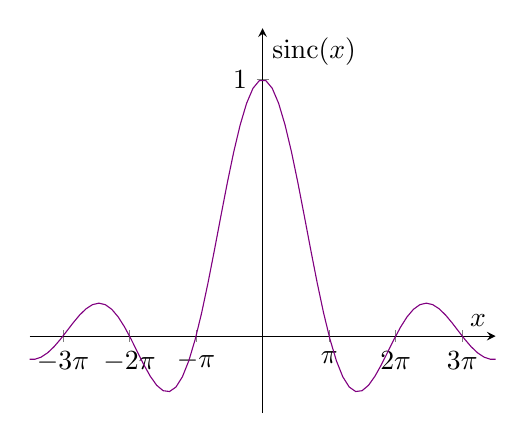
\begin{tikzpicture}
\begin{axis}[
    width=7.5cm,
    % grid=both,
    xmin=-11,
    xmax=11,
    ymin=-0.3,
    ymax=1.2,
    xlabel=$x$,
    ylabel=$\mathrm{sinc}(x)$,
    axis lines=center,
    xticklabels={$-3\pi$, $-2\pi$, $-\pi$, $\pi$, $2\pi$, $3\pi$},
    xtick={-3*3.141592, -2*3.141592, -3.141592, 3.141592, 2*3.141592, 3*3.141592},
    ytick={0, 1}
]
  \addplot[
    domain=-15:15,
    violet,
    ultra thick,
    samples=100,
  ] plot[thin] {sin(deg(x))/x};
\end{axis}
\end{tikzpicture}
\end{marginfigure}

\begin{preuve}
    \begin{enumerate}
        \item Montrer que $\int_{0}^{1} \frac{\sin (t)}{t} \d t$ est convergente. 
        \item Deux méthodes.
        \begin{itemize}
            \item Montrer que la série de terme général $\int_{n \pi}^{(n+1) \pi} \frac{\sin(t)}{t} \d t$ est convergente. En déduire que $\int_{1}^{+ \infty} \frac{\sin(t)}{t} \d t$ converge. 
            \begin{enumerate}
                \item Montrer que $u_n = \int_{n \pi}^{(n+1) \pi} \frac{\sin(t)}{t} \d t$ est le terme général d'une série alternée. Donc $\sum u_n$ converge.\\
                Attention: on ne peut pas en déduire directement que $\sum\limits_{n=0}^{+ \infty} \int_{n \pi}^{(n+1) \pi} \frac{\sin(t)}{t} \d t = \int_{1}^{+ \infty} \frac{\sin(t)}{t} \d t$ car on n'a pas encore démontré la convergence du deuxième membre (c.f. relation de \textsc{Chasles}).\\
                \item Il faut montrer la convergence de $\int_{\pi}^{x} \frac{\sin (t)}{t} \d t$. \textcolor{green}{A compléter.}
            \end{enumerate}
            \item On peut aussi procéder par intégration par parties en posant
            $$
            \begin{drcases}                
                u(t) = \frac{1}{t}\\
                v(t) = - \cos(t)
            \end{drcases}
            \mathscr{C}^1 \text{ sur } [1, +\infty].
            $$
            Bien présicer que $u(t)v(t)=-\frac{\cos(t)}{t}$ admet une limite finie en 1 et en $+ \infty$.\\
            \begin{remarque}
                L'intégration par parties préserve la régularité de l'intégrale mais ne préserve pas l'intégrabilité.
            \end{remarque}
        \end{itemize}
        \item On en déduit immédiatement que $\int_{0}^{+ \infty} \frac{\sin (t)}{t} \d t$ converge.
        \item De plus, on peut montrer que cette intégrale est semi-convergente (i.e. elle n'est pas intégrable sur $\Rp$). Pour cela, montrer que pour tout entier naturel $n$, $\int_{n \pi}^{(n+1) \pi} \frac{\sin(t)}{t} \d t \geqslant \frac{2}{(n+1) \pi}$. 
    \end{enumerate}
\end{preuve}

\subsection{Intégrabilité du sinus cardinal sur  \texorpdfstring{$\Rpe$}{R+*}}

\begin{prop}{}
    La fonction sinus cardinal $\mathrm{sinc}:t \mapsto \frac{\sin(t)}{t}$ n'est pas intégrable sur $]0, +\infty[$.
\end{prop}

\begin{preuve}
    \marginnote[0cm]{Source : \href{https://www.agreg-maths.fr/uploads/versions/1175/dirichlet.pdf}{Intégrale de \textsc{Dirichlet} -- Florian \textsc{Dussap}}}
    Soit $N \in \Ne$, alors:
    \begin{align*}
        \int_0^{N \pi} \frac{|\sin x|}{x} \d x &= \sum_{k=0}^{N-1} \int_{k \pi}^{(k+1) \pi} \frac{|\sin x|}{x} \d x \\
        \text{par un changement de variable } &= \sum_{k=0}^{N-1} \int_0^\pi \frac{|\sin x|}{x + k \pi} \d x \\
        &\geqslant \sum_{k=0}^{N-1} \frac{1}{(k+1) \pi} \int_0^\pi \sin x \d x \\
        &\geqslant \frac{2}{\pi} \sum_{k=1}^N \frac{1}{k} \xrightarrow[N \to + \infty]{} + \infty.
    \end{align*}
\end{preuve}

\subsection{Intégrale de \textsc{Dirichlet} via une intégrale à paramètre}

Soit la transformée de \textsc{Laplace} de la fonction sinus cardinal:
$$F:x \to \int_{0}^{+ \infty} \exp(-xt) \frac{\sin (t)}{t} \d t$$
    
\begin{enumerate}
    \item \emph{Montrer que $F$ est définie sur $\Rp$.}
    \begin{itemize}
        \item Si $x > 0$, majorer l'intégrande par $t \mapsto \exp(-xt)$.
        \item Si $x = 0$, montrer le prolongement par continuité de la fonction sinus cardinal en $0$ puis intégrer la fonction sinus cardinal par parties sur $[1, +\infty]$.
    \end{itemize}
    \item \emph{Calculer $F$ sur $\Rpe$, en déduire la valeur de la fonction de \textsc{Dirichlet}}
\end{enumerate}

\subsection{Régularité du sinus cardinal sur $\R$}

\begin{exercice}
    Pour $x$ réel, on pose 
    $$f(x) \defeq
    \begin{cases} 
        \frac{\sin x}{x} &\text{si } x \not= 0 \\ 
        1 &\text{si } x = 0 
    \end{cases}.$$ 
    Montrer que $f$ est de classe $\mathscr{C}^\infty$ sur $\R$.
\end{exercice}

\begin{solution}
    \marginnote[0cm]{fic00126}
    Pour $x$ réel non nul, $f(x) = \sum\limits_{n=0}^{+ \infty} (-1)^n \frac{x^{2n}}{(2n+1)!}$ ce qui reste vrai pour $x = 0$. La fonction $f$ est donc développable en série entière sur $\R$ et en particulier, la fonction $f$ est de classe $\mathscr{C}^\infty$ sur $\R$.
\end{solution}

\todoarmand{Énoncés issus de bestiaire.pdf}

\begin{exercice}
    Exercice 167 p.179 \\
    On considère l'application $f(x) = \int_0^\infty \frac{\sin(t)}{t} \e^{-xt} \d t$.
    \begin{enumerate}
        \item Montrer que $f \in \mathscr{C}^1(\Rpe)$.
        \item En déduire une forme explicite de $f$ sur $\Rpe$. 
        \item Montrer que $f$ est continue à l'origine. 
        \item En déduire que $\int_0^\infty \frac{\sin(t)}{t} \d t = \frac{\pi }{2}$.
    \end{enumerate}
\end{exercice}

\begin{exercice}
    Exercice 170 p. 184 \\
    Soient $f(x) = \int_0^\infty \frac{\sin(t)}{t+x} \d t$, $g(x) = \int_0^\infty \frac{\e^{-xt}}{t^2 + 1} \d t$. 
    \begin{enumerate}
        \item Montrer que $f, g \in \mathscr{C}^2(\Re)$. \\
        \textit{Pour $f$, on pourra commencer par montrer que $f(x) = \int_0^\infty \frac{1 - \cos(t)}{(t+x)^2} \d t$.}
        \item Montrer que $f$ et $g$ sont solutions de l'équation différentielle $y'' + y + \frac{1}{x}$.
        \item En déduire que $f-g$ est $2 \pi$-périodique (sur son domaine de définition).
        \item Montrer que $f$ et $g$ sont équivalentes à $\frac{1}{x}$ en $+\infty$ puis, que $f = g$.
        \item En déduire la valeur de $\int_0^\infty \frac{\sin(t)}{t} \d t$.
    \end{enumerate}
\end{exercice}

\todoinline{J'ai mis ENSAIT - MP - 96 dans les documents. On l'ajoute ici ?}

\todoarmand{Pourquoi pas, on pourrait sélectionner l'une des parties, le III par exemple.}